\chapter{Voice Activity Detection}
\label{sec:vad}

Das Ziel ist, in einem Audiosignal diejenigen Stellen zu markieren, in denen Stimme enthalten ist. Abbilung \ref{img:vad01} visualisiert ein Beispiel für eine solche Markierung. Zu sehen ist der Zeitbereich eines Audiosignales mit fünf klar erkennbaren Cry-Units. Die rote Linie, die das Signal überspannt, bildet die Zeiteinheiten des Eingangssignales in die binären Kategorien $1 hat{=} $ \emph{stimmhaft} (engl. \emph{voiced}) und $0 hat{=}  $ \emph{Stille} (oder \emph{nicht-stimmhaft}, engl. \emph{not voiced}) ab.

\begin{figure}[h]
	\centering
	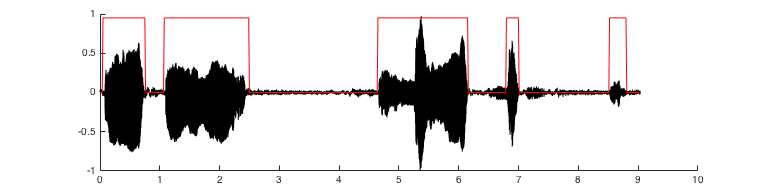
\includegraphics[width=0.7\textwidth]{bilder/vad_introduction01.png}
	\caption{Markierung stimmhafter Bereiche in einem Audiosignal. Schwarz: Das Eingangssignal $x[\;]$. Rot: Klassifizierung in stimmhaft/Stille. Es sind fünf Cry-Units zu erkennen.}
	\label{img:vad01}
\end{figure}

Die Erkennung des Vorhandenseins von Stimme in einem Signal wird als \emph{Voice Activity Detection (VAD)} oder auch \emph{Speech Detection} bezeichnet. Das Ziel ist die Unterscheidung von denjenigen Zeiträumen im Signal, in denen Stimme enthalten ist, von den Zeiträumen ohne Stimme. Die größte Herausforderung für VAD-Algorithmen ist die robuste Erkennung bei Signalen mit Rauschen unbekannter Stärke und Natur. \cite[S. 1]{vad_kola} \cite[S. 1]{vad_Lisboa}

Der Grundlegende Aufbau eines VAD-Algorithmus ist wie folgt.
\begin{enumerate}
\item \textbf{Windowing:} Unterteilung des Signals in (einander überlappende) Signalfenster.
\item \textbf{Extraktion von Eigenschaften} aus den einzelnen Signalfenstern.
\item \textbf{Entscheidung} über die Präsens oder Abwesenheit von Stimme für jedes Signalfenster auf Grundlage der extrahierten Attribute mit Hilfe von Entscheidungsregeln wie Grenzwerten.
\item \textbf{Decision-Smoothing}, das nachträgliche Hinzufügen oder Entfernen von Entscheidungen mit Hilfe von kontextuellen Informationen der umliegenden Entschiedungen.\cite[S. 8 - 9]{vad_granada} \cite[S. 1 - 2]{vad_kola}
\end{enumerate}

Auch die in dieser Arbeit durchgeführte Voice Activity Detection folgt diesem Schema. Das Windowing wird in Kapitel \ref{sec:windowing}, die Extraktion von Eigenschaften in Kapitel \ref{sec:featExtraction}, die Entscheidung in Kapitel \ref{sec:vad_thresholding} und das Decision-Smoothing in Kapitel \ref{sec:smoothing} beschrieben. Es wurden Ideen verwendet, die von  Moattar et al. \cite{vad_Easy}, Kristjansson et al. \cite{vad_Lisboa}, Waheed et al. \cite{vad_entropy}, Ahmadi et al. \cite{vad_ceps} und Shen et al.\cite{vad_entropie02} vorgestellt wurden.

\subsection{Windowing}
\label{sec:windowing}

Wird die Voice Activity Detection für ein Signal $x[\;]$ durchgeführt, wird dieses zuerst nach dem in Kapitel \ref{sec:stft} beschriebenen Verfahren nach Gleichung \ref{eq:signal-Window} in die Signalfenster $x_0[\;] , \ldots , x_m[\;]$ zerlegt. Der Prozess wird als \glqq Windowing\grqq{} bezeichnet. Die Signalfenster werden zunächst im Zeitbereich belassen. Es wurde sich für die von Waheed et al. \cite{vad_entropy} vorgeschlagene Fensterlänge von \SI{25}{\milli\second} entschieden, als Kompromiss zwischen den von Moattar et al\cite{vad_Easy} empfohlenen \SI{10}{\milli\second} und den von Ahmadi et al \cite{vad_ceps} empfohlenen \SI{40}{\milli\second}. Die Fenster überlappen einander um 50\%, das heißt \SI{12.5}{\milli\second}.

\subsection{Extraktion von Eigenschaften}
\label{sec:featExtraction}

Um die Entscheidung zu treffen, ob in einem beim Windowing enstandenen Signalfenster $x_i[\;]$ Stimme enthalten ist, wird zunächst eine Reihe an Eigenschaften für das Signalfenster berechnet. Auf Basis dieser Eigenschaften kann daraufhin die Entscheidung gefällt werden. Einer der primären Forschungsgegenstände der VAD ist die Erprobung und Evaluation von Eigenschaften zu diesem Zweck. In diesem Kapitel wird eine Reihe an Attribute vorgestellt, mit dem Ziel, diejenigen zu identifizieren, die sich im Zusammenhang mit kindlichen Lautäußerungen am besten zur Erkennung von Stimme eignen. Das Vorgehen ist folgendermaßen:

\begin{enumerate}
	\item Es wurde ein Testdatensatz mit Audioaufnahmen von kindlichen Lautäußerungen erstellt. Diese Datensätze werden in Kapitel \ref{sec:databases} beschrieben.
	\item Jedes Signal des Datensatzes wurde nach dem eben beschriebenen Vorgehen vorverarbeitet und daraufhin in kürzere Signalfenster zerlegt. Für jedes Signalfenster wurden die Eigenschaften berechnet, die in den folgenden Kapiteln \ref{sec:timeFeats} bis \ref{sec:theFeatureSpace} beschrieben werden.
	\item Das Ziel war es, eine möglichst kleine Untermenge an Eigenschaften zu finden, auf deren Basis die Entscheidung über das Vorhandensein von Stimme mit einer möglichst hohen Genauigkeit durchgeführt werden kann. In Kapitel \ref{sec:vad_thresholding} wird beschrieben, wie die verschiedenen Eigenschaften bezüglich ihrer Performance evaluiert wurden.
\end{enumerate}

Für jedes Signalfenster $x_i[\;]$ à \SI{25}{\milli\second} des Testdatensatzes wurden die folgenden Features aus den Kategorien \textbf{Zeitbereich}, \textbf{Frequenzbereich}, \textbf{Cesptrum} und \textbf{Autokorrelation} erprobt. 

\subsubsection{Zeitbereich}
\label{sec:timeFeats}

Im Zeitbereich wurden die beiden Eigenschaften\emph{Root Mean Square} [\emph{RMS}] und \emph{Zero Crossing Rate} [\emph{ZCR}] berechnet.

Moattar et al. \cite{vad_Easy} bezeichnen den Energiegehalt eines Signals als das für die VAD am häufigsten angewandte Attribut. Daher wurde der RMS-Wert nach Gleichung \ref{eq:rms} für die Signalfenster berechnet. Hintergrund ist, dass der Energiegehalt eines Stimmsignals typischerweise höher ist als der des Hintergrundrauschens. Bei geringem Signal/Rauschabständen ist diese Bedingung jedoch nicht immer gegeben. Als zweites Attribut des Zeitbereiches wurde die \emph{Zero Crossing Rate} berechnet. Die ZCR nach Formel \ref{eq:zcr} gibt an, wie häufig ein Vorzeichenwechsel im Signal vorkommt. Eine höhere ZCR weist auf Stille hin, da Rauschen typischerweise eine höhere ZCR als stimmhafte Signale aufweist. Problematisch ist dieses Kriterium bei Signalen, bei denen kein Hintergrundrauschen vorliegt, da sich dort eine ZCR von 0 ergibt.\cite{vad_ceps} Um den Wert in Relation zur Fensterlänge setzen zu können, wurde weiterhin die ZCR durch die Anzahl der Samples eines Signalfensters $N$ geteilt.

\begin{equation}
\text{ZCR}(x_i[\;]) = \sum_{0}^{N-1}|\text{sng}(x_i[n])-\text{sng}(x_i[n-1])|
\label{eq:zcr}
\end{equation}

\subsubsection{Autokorrelation}

Neben den in Kapitel \ref{sec:featExtraction} genannten \glqq einfachen\grqq{} Attributen des Zeitbereiches wurde die Autokorrelation erprobt. Wie in Kapitel \ref{sec:theVoice} ausgeführt, weisen stimmhafte Signale eine tendenziell stärkeres periodisches Verhalten als das Hintergrundrauschen auf. Daher eignet sich die in Kapitel \ref{sec:autocorrelation} vorgestellte Autokorrelation, um diese Periodizität festzustellen. Es wurden die Attribute \emph{Maximum Autocorrelation Peak} [\emph{aMax}] und (\emph{Autocorrelation Peak Count}) [\emph{aCount}] berechnet. 

Beide Eigenschaften wurden von Kristjansson et al. \cite[S. 1 - 2]{vad_Lisboa} zur VAD beschrieben. Die (\emph{Maximum Autocorrelation Peak}) wird in Formel \ref{eq:corrpeak} definiert und bestimmt die höchste Magnitude im Autokorrelationssignal. Eine hoher [\emph{aMax}]-Wert weist auf eine starke Periodizität hin. Das zweite Attribut ist die \emph{Autocorrelation Peak Count} nach Formel \ref{eq:corrcount}. Dabei wird die Anzahl an Signalspitzen im Autokorrelationssignal gezählt. Rauschen erzeugt höhere [\emph{aCount}]-Wert als stimmhafte Signale, bedingt durch die vielen zufällig Verteilten Periodizitäten. Aus Kapitel \ref{sec:acousticModel} ging hervor, dass die Grundfrequenz der Stimme von Neugeborenen zwischen $200$ und $\SI{2000}{\hertz}$ liegt, weshalb auch nur in Lags dieses Bereichs verwendet wurden.

\begin{equation}
\text{aMax}(x_i[\;]) = \max_{k}\text{mag}\{\text{NA-Corr}_k(x_i[\;])\}
\label{eq:corrpeak}
\end{equation}

\begin{equation}
\text{aCount}(x_i[\;]) = \counti_{k}\text{mag}\{\text{NA-Corr}_k(x_i[\;])\}
\label{eq:corrcount}
\end{equation}


\subsubsection{Frequenzbereich}

Aus dem Frequenzbereich wurden die drei Eigenschaften \emph{unnormalisierte spektrale Entropie} [$SEnt_{u}$], \emph{normalisierte spektrale Entropie}  [$SEnt_{n}$] und \emph{dominanteste Frequenzkomponenten} [$f_{dom}$] berechnet.

Als Vorbereitungsschritt muss das Signalfenster des Zeitbereiches $x_i[\;]$ in den Frequenzbereich $X_i[\;]$ transformiert werden. Die Berechnungsvorschrift ist $X_i[\;] = \text{DFT}\{(w[\;] \cdot x_i[\;])\}$. Wird diese Transformation für alle Signalfenster $x_0[\;], \ldots, x_m[\;]$ eines Signals durchgeführt, entspricht dies der in Kapitel \ref{sec:stft} vorgestellten Short Time Fourier Transformation. Es wurde eine $2048$ Punkte Lange FFT und eine Hamming-Window als Fensterfunktion $w[\;]$ verwendet.

Kristjansson et al. \cite[S. 2]{vad_Lisboa} haben die \emph{spektrale Entropie} zur Voice Activity Detection beschrieben. Dabei wird das Spektrum des Frequenzfensters $X_i[\;]$ als Wahrscheinlichkeitsverteilung betrachtet. Die Entropie als Maß zur \glqq Unreinheit\grqq{} wurde in Kapitel \ref{sec:id3} erläutert. Die \emph{normalisierte spektrale Entropie} wird nach der Formel \ref{eq:norm_se} berechnet. Das Signal $px_i[\;]$ ergibt sich durch die Normalisierung des $N$-Punkte langen Spektrums nach Formel \ref{eq:norm_spek}. Neben der von Kristjansson et al. \cite{vad_Lisboa} vorgestellten normalisierten spektralen Entropie wurde zusätzlich die \emph{unnormalisierte Spektrale Entropie} nach Formel \ref{eq:unnnorm_se} berechnet. Bei dieser wird das Spektrum nicht normalisiert, das heißt, es gilt $px_i[k] = X_i[k]$. Somit hat die Energie des Signals einen größeren Einfluss den Wert des Attributes. Bei der normalisierten spektralen Entropie ist zu erwarten, dass Frequenzfenster ohne Stimme einen höheren Wert aufweisen als Fenster mit Stimme. Bei der unnormalisierten spektralen Entropie ist zu erwarten, dass Signalfenster mit Stimme einen höheren Wert aufweisen als Signale mit Stille.\footnote{Kristjansson et al \cite[S. 2]{vad_Lisboa} verwenden zur Entropie-Berechnung den Logarithmus zur Basis 10, anstatt zur Basis 2. Es ist nicht klar, ob es sich dabei um einen Fehler handelt. In dieser Arbeit wurde, wie in dem Paper beschrieben, ebenfalls der Logarithmus zur Basis 10 verwendet!}

In die Berechnungen wurden nur die Frequenzen im Bereich von 200 - \SI{8000}{\hertz} mit einbezogen, da nach Kapitel \ref{sec:acousticModel} die tiefst mögliche Frequenz der Stimme eines Babys bei \SI{200}{\hertz} liegt und nach Shen et al. \cite{vad_entropie02} die Stimme keine Informationen oberhalb von \SI{8000}{\hertz} enthält.

\begin{equation}
px_i[n] = \frac{X_i[n]}{\sum_{k=1}^{N} X_i[k]}
\label{eq:norm_spek}
\end{equation}

\begin{equation}
\text{SEnt}_n(px_i[\;]) = -\sum_{k=1}^{N}px_i[k] \cdot\log(px_i[k])
\label{eq:norm_se}
\end{equation}

\begin{equation}
\text{SEnt}_u(X_i[\;]) = -\sum_{k=1}^{N}X_i[k] \cdot\log(X_i[k])
\label{eq:unnnorm_se}
\end{equation}

Moattar et al \cite[S. 2550]{vad_Easy} haben die \emph{dominanteste Frequenzkomponente} zur Voice-Activity-Detection vorgestellt. Für jedes Frequenzfenster $X_i[\;]$ wird diejenige Frequenz nach Formel \ref{eq:domfreq} berechnet, welche die höchste Amplitude hat. Es wird dabei, im Gegensatz zur spektralen Entropie, der gesamte Frequenzraum betrachtet. Ein stimmhaftes Signal hat typischerweise eine höhere $f_{dom}$ als ein stimmloses Signal, bedingt durch die hohe Amplitude der Grundfrequenz.

\begin{equation}
f_{dom}(X_i[\;]) = \argmax \{X_i[\;]\}
\label{eq:domfreq}
\end{equation}


\subsubsection{Cepstrum}
\label{sec:cepstrum-feature}

In Kapitel \ref{sec:autocorrelation} wurde das Cepstrum vorgestellt und erläutert, wie Peaks im oberen Quefrency-Bereich auf das Vorhandensein eines periodischen, obertonreichen Signals, wie zum Beispiel Stimme, hinweisen. Aus dem Cepstrum-Bereich wurden die Features \emph{Upper Cepstrum Peak} [$Ceps_{mag}$] und \emph{Upper Cepstrum Peak Location} [$Ceps_{loc}$] berechnet.

Ahmadi et al. \cite{vad_ceps} sowie Kristjansson et al.\cite{vad_Lisboa} schlagen vor, die höchste Magnitude im oberen Quefrency-Bereich (Upper Cepstrum Peak) als Feature zu verwenden. Formel \ref{eq:ceps_maxpeak} definiert die Berechnung. $c_i[\;]$ ist das Cepstrum des $i$-ten Frequenzfensters $X_i[\;]$. Wie in Kapitel \ref{sec:acousticModel} erläutert, liegt die Grundfrequenz bei kindlichen Lautäußerungen zwischen 200 und \SI{2000}{\hertz}, was einem Quefrency-Bereich von 5 - \SI{40}{\milli\second} entspricht. Folglich werden bei der Berechnung nach Formel \ref{eq:ceps_maxpeak} nur Quefrency-Werte in diesem Bereich betrachtet. Ein hoher $Ceps_{mag}$-Wert weist auf das Vorhandensein von Stimme hin. Als zweites Attribut wird die Quefrency der höchsten Amplitude des Cepstrum (Upper Cepstrum Peak Location) nach Formel \ref{eq:ceps_loc} berechnet. Bei Signalfenstern mit Stille ist es wahrscheinlicher, dass sich die höchste Amplitude am Mindest- oder Maximalwert des durchsuchten Quefrency-Bereiches befindet.

\begin{equation}
Ceps_{mag}(c_i[\;]) = \max\text{mag}\{c[\;]\}
\label{eq:ceps_maxpeak}
\end{equation}

\begin{equation}
Ceps_{loc}(c_i\;) = \argmax \{c[\;]\}
\label{eq:ceps_loc}
\end{equation}

Abbildung \ref{img:vadAllFeatures} visualisiert alle vorgestellten Attribute, die für die Voice Activity Detection erprobt wurden. Der oberste Plot zeigt das Audiosignal aus Abbildung \ref{img:vad01} mit einem Signal/Rausch-Abstand von \SI{20}{\decibel}. Der rote Graph über dem Plot klassifiziert die Zeitbereiche in $1 \hat{=} $ \emph{stimmhaft} und $0 \hat{=}$ \emph{nicht stimmhaft}. Alle darunter liegenden Plots zeigen den zeitlichen Verlauf der entsprechenden Attribute.

\begin{figure}[h!]
	\centering
	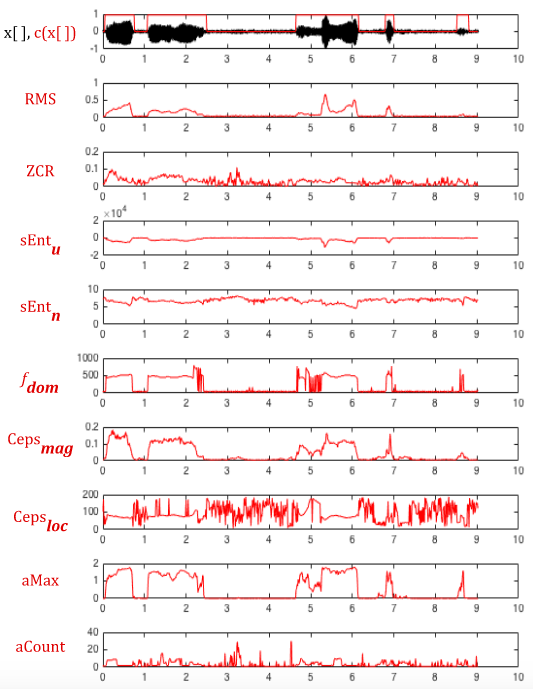
\includegraphics[width=1\textwidth]{bilder/allFeatures01.png}
	\caption{Übersicht über alle Features, die für die Voice Activity Detection erprobt wurden.}
	\label{img:vadAllFeatures}
\end{figure}

\subsubsection{Konstruktion des Feature-Raumes}
\label{sec:theFeatureSpace}

Abbildung \ref{img:min-signal} zeigt in (A) des zeitlichen Verlauf des \emph{RMS}-Attributes eines Signals mit einem Signal/Rauschabstand von \SI{50}{\decibel}. Die Zeiträume mit Stille haben einen weitaus niedrigeren RMS-Wert als die Zeiträume mit Stimme. In (B) ist das selbe Signal mit einem Signal/Rauschabstand von \SI{3}{\decibel} zu sehen. Nun liegen die RMS-Werte der stimmlosen Bereiche nur noch knapp unter denen des Sprachsignals. Zu sehen ist, dass starkes Hintergrundrauschen ähnlich hohe Feature-Werte erzeugen kann wie die Stimme.

\begin{figure}[h]
	\centering
	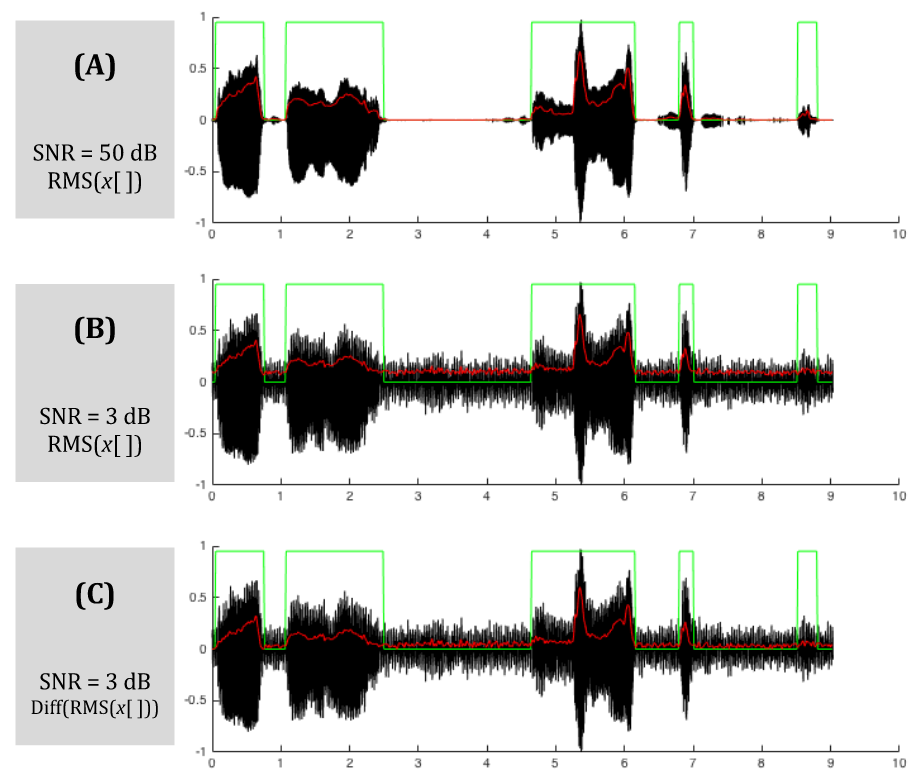
\includegraphics[width=0.7\textwidth]{bilder/rms_diff.png}
	\caption{Das RMS-Feature bei verschiedenen Signal/Rausch-Abständen. Schwarz: Eingangs-Signal $x[\;]$. Grün: Klassifizierung in Stimmhaft/Stille. Rot: Feature-Wert.}
	\label{img:min-signal}
\end{figure}

Moattar et al \cite{vad_Easy} und Waheed et al \cite{vad_entropy} präsentierten die Idee, den Wert des jeweiligen Attributes zu messen, der in den stimmlosen Bereichen durch das Hintergrundrauschen erzeugt wird. Es kann davon ausgegangen werden, dass die ersten Signalfenster eines Signals zunächst noch keine Stimme enthalten, und der Feature-Wert des Rauschens somit anhand dieser Fenster bestimmt werden kann. Bei einer langanhaltenden und kontinuierlichen Analyse können sich sowohl die Signal/Rauschabstände als auch die Qualität des Rauschens ständig ändern, weshalb die von den stimmlosen Bereichen erzeugten Attributwerte regelmäßig aktualisiert werden müssen. Es kann weiterhin davon ausgegangen werden, dass die Länge einer Cry-Unit eine bestimmte Länge $t_{max}$ nicht überschreiten kann, bevor das Baby Luft holen muss und somit ein Zeitfenster mit Stille entsteht. Zeskind et al. \cite[S. 325]{rythmic} haben diesen Wert mit $t_{max} = \SI{4.75}{\second}$ bestimmt. In einem Zeitbereich $ t > t_{max}$ muss somit zumindest ein Feature-Wert enthalten sein, der durch stimmlose Signalteile erzeugt wird. Auf Basis dieser Überlegung wird das \emph{Differenz-Feature} Diff\textsubscript{t}(Feat$(x_i[\;])$) nach Formel \ref{eq:difFeature} definiert als die Differenz zwischen dem aktuell gemessenen Attributwerte und dem geringsten Attributwerte, welcher im vergangenen Zeitbereich $t$ gemessen wurde. Feat$(x_i[\;])$ bezeichnet dabei einen beliebigen Feature-Wert des Signalfensters $x_i[\;]$, $t_{xi}$ die Länge eines Signalfensters in Sekunden (in diesem Fall \SI{25}{\milli\second}), und $t$ der in der Vergangenheit zu durchsuchende Zeitbereich in Sekunden $> t_{max}$. In Abbildung \ref{img:min-signal} wird in (C) das Differenz-Feature für den RMS-Wertes gezeigt.

\begin{equation}
\text{Diff}_t(\text{Feat}(x_i[\;])) = Feat(x_i[\;])\ - \mini_{k=i-z...i}\{Feat(x_k[\;])\}, \qquad z = \frac{2 \cdot t}{t_{xi}}
\label{eq:difFeature}
\end{equation}

Der Feature-Raum wurde schlussendlich folgendermaßen zusammengesetzt: Die ersten 9 Features bildeten die in Attribute \emph{RMS, ZCR, SEnt\textsubscript{u}, SEnt\textsubscript{n}, $f_{dom}$, Ceps\textsubscript{mag}, Ceps\textsubscript{loc}, aMax} und \emph{aCount}. Weiterhin wurde für jedes Attribut nach Formel \ref{eq:difFeature} das Differenz-Feature mit $t = \SI{5}{\second}$ berechnet. Die Features \emph{ZCR, SEnt\textsubscript{u}} und \emph{aCount} wurden vor der Berechnung des Differenz-Features bezüglich ihres Vorzeichens invertiert, da bei Ihnen ein niedriger anstatt ein hoher Wert stimmhafte Signale anzeigen. Das einzige Attribut, für den kein Differenz-Feature berechnet wurde, ist das \emph{Ceps\textsubscript{loc}}-Attribut, da es bei Stille sowohl einen höheren als auch einen niedrigeren Wert annehmen kann. Der Feature-Raum umfasste somit insgesamt $9 + 8 = 17 $ Dimensionen. Gleichung \ref{eq:featureVektor} verdeutlicht die Zusammensetzung des Feature-Vektors $v_i$, der für das Signalfenster $x_i[\;]$ berechnet wurde.

\begin{equation}
v_i = \Big( \text{RMS}(x_i[\;]), ...,\text{ aCount}(x_i[\;]), 
\text{Diff}_{t}(\text{RMS}(x_i[\;])) .... \text{Diff}_{t}(-\text{ aCount}(x_i[\;]))\Big)
\label{eq:featureVektor}
\end{equation}

\subsection{Thresholding}
\label{sec:vad_thresholding}

\subsubsection{Finden der Grenzwerte}

Das Ziel war es nun, Grenzwerte für die Attribute zu finden, bei deren Über- oder Unterschreitung das jeweilige  Signalfenster als \emph{stimmhaft} klassifiziert wird. Abbildung \ref{img:thresholded} verdeutlicht das Prinzip für das \emph{RMS}-Attribut. Diese Entscheidung nach einem Grenzwert ist ein klassisches Vorgehen bei der Voice-Activity-Detection. Eine binäre Klassifizierung nach dem Muster $C(x_i[\;]) = \{ 1, \text{wenn } \text{RMS}(x_i[\;]) \geq 0.18 ,\quad 0 \text{ sonst}\}$ würde in diesem Fall eine weitestgehend richtige Klassifizierung vornehmen.

\begin{figure}[h]
	\centering
	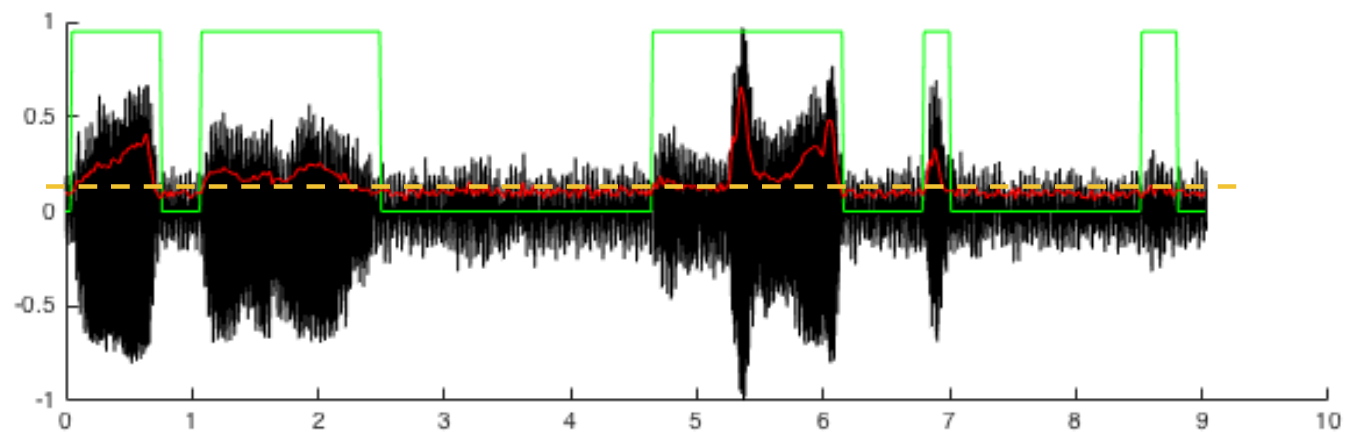
\includegraphics[width=0.6\textwidth]{bilder/thresholded02.png}
	\caption{Thresholding eines Features. Schwarz: Das Eingangssignal $x[\;]$. Grün: Klassifizierung in Stimmhaft/Stille. Rot: RMS-Feature. Orange: Grenzwert}
	\label{img:thresholded}
\end{figure}

Eine Methode zum Finden der optimalen Grenzwerte ist der in Kapitel \ref{sec:c45} vorgestellte \emph{C4.5}-Algorithmus. Da der \emph{C4.5}-Algorithmus Entscheidungsbäume erstellt, kann die Entscheidung über das Vorhandensein von Stimme in einem Signalfenster aufgrund der Verkettung von Grenzwerten mehrerer Attribute in Folge gefällt werden. Ein Beispiel wird in Listing \ref{lst:tree01} dargestellt, bei dem die Klasse eines  Signalfensters hierarchisch zuerst nach einem Grenzwert für Ceps$_{mag}$ und danach für den RMS-Wert entschieden wird.

\begin{lstlisting}[frame=single,mathescape=true,basicstyle=\footnotesize,language=Java,label=lst:tree01,caption=Beispiel eines CART-Entscheidungsbaums,linewidth=1\textwidth]
if Ceps$_{mag}$($x_i[\;]$) > 0.2
|   if RMS($x_i[\;]$) < 0.13
|   |   C($x_i[\;]$) = 0
|   |else
|   |   C($x_i[\;]$) = 1
|else
|    C($x_i[\;]$) = 1
\end{lstlisting}

\subsubsection{Trainings- und Testdatensätze}
\label{sec:databases}

Es wurden sechs Audioaufnahmen mit Weinen verschiedener Babies von der freien Online-Sound-Bibliothek \url{https://www.freesound.org/} heruntergeladen und zu Segmenten \`{a} \SI{10}{\second} beschnitten. Es handelt sich um weitgesgehend rauschfreie Aufnahmen, die von verschiedenen Babys stammen. In den Audiosignalen wurden manuell die Zeitbereiche markiert, welche Stimme enthalten. Es wurden \emph{keine} Geräusche markiert, bei denen es sich offensichtlich um Einatumungs-Geräusche handelt. Geräusche, bei denen nur Anhand der Aufnahme nicht mit Sicherheit festgestellt werden konnte, ob es sich um Einatmungs- oder Ausatmungsgeräusche handelt, wurden als Stimme markiert. Weiterhin wurden drei verschiedene Rauschsignale heruntergeladen. Es handelt sich um \glqq realistische\grqq{} Atmosphären von Krankenhäusern. Jedes der sechs Audioaufnahmen der Babys wurde mit jedem der drei Rauschsignale überlagert, einmal mit einem Signal/Rausch-Abstand von \SI{50}{\decibel} (\glqq fast unhörbares Rauschen\grqq), und einmal mit einem Signal/Rausch-Abstand von \SI{3}{\decibel} (\glqq starkes Rauschen\grqq). Außerdem wurde ein siebte Aufnahme eines Babys heruntergeladen, welches mit einem vierten Rauschsignal mit einem SNR von \SI{7}{\decibel} überlagert wurde. Dieses Signal spielt eine Sonderrolle, da es nur zur Verifikation verwendet wird. So wurden vier Mengen an Audiosignalen erzeugt:

\begin{description}
	\item[A\textsubscript{\SI{50}{\decibel}}] enthält $3 \cdot 6 = 18$ Audiosignale, bei dem alle sechs Baby-Aufnahmen mit den drei Rauschsignalen bei einem Signal/Rausch-Abstand von \textbf{\SI{50}{\decibel}} überlagert wurden
	
	\item[A\textsubscript{\SI{3}{\decibel}}] enthält $3 \cdot 6 = 18$ Audiosignale, bei dem alle sechs Aufnahmen der Babys mit den drei Rauschsignalen bei einem Signal/Rausch-Abstand von \textbf{\SI{3}{\decibel}} überlagert wurden
	
	\item[A\textsubscript{50+\SI{3}{\decibel}}] $ = \{ A_{\SI{50}{\decibel}} \cup  A_{\SI{3}{\decibel}}\} = 32$ Audiosignale
	
	\item[A\textsubscript{\SI{7}{\decibel}*}] enthält $1$ Audiosignal, bei dem eine siebte Aufnahme eines Babys mit einem vierten Rauschsignal bei einem Signal/Rausch-Abstand von \textbf{\SI{7}{\decibel}} überlagert wurde
	
\end{description}

Im nächsten Schritt werden die eigentlichen Datensätze $D_{SNR,Feats}$ gebildet, in dem Audiosignale dieser Signalmengen (1) wie in Kapitel \ref{sec:preprocessing} beschrieben vorverarbeitet werden, (2) wie in Kapitel \ref{sec:windowing} in die Signalfenster \`{a} \SI{25}{\milli\second} zerlegt werden und (3) für jedes Signalfenster der durch Gleichung \ref{eq:featureVektor} definierte Featurevektoren berechnet wird. Außerdem wird jedem Featurevektor die Klasseninformation \emph{Stimme/Stille} zugewiesen.

Es ist rechnerisch zu aufwendig, alle genannten Features in einem kontinuierlichen System zur Voice Activity Detection zu berechnen. Daher werden die Datensätze in Untermengen bezüglich der verwendeten Features eingeteilt. Das Ziel ist es, eine möglichst kleine Untermenge an Features zu finden, die sich am besten für die Voice Activity Detection sowohl bei niedrigem als auch bei starkem Hintergrundrauschen eignet. Die Untermengen werden in Bezug auf die Methode gebildet, durch die die Features berechnet werden. Das heißt, dass beispielsweise die Untermenge \emph{Zeit} die in Kapitel \ref{sec:timeFeats} beschriebenen Features \emph{RMS} und \emph{ZCR} sowie die dazugehören Differenzfeatures \emph{Diff\textsubscript{t}(RMS)} und \emph{Diff\textsubscript{t}(ZCR)} beinhaltet. 

Die 9 Untermengen sind: \{ Zeitbereich, Frequenzbereich, Cepstrum, Autokorrelation, Zeit + Frequenzbereich, Zeit + Cepstrum, Zeit + Autokorrelation, Frequenzbereich + Cepstrum, Frequenzbereich + Autokorrelation \}. Cepstrum- und Autokorrelation werden nicht gemeinsam in eine Untermenge hinzugefügt, da sie in Bezug auf den Berechnungsaufwand die aufwendigsten sind. So enthält beispielsweise der Datensatz $D_{\SI{3}{\decibel},Zeit}$ die Featurevektoren des Zeitbereiches für die Audiosignale mit einem Signal-Rausch-Abstand von \SI{3}{\decibel}. Alle Audiosignal-Mengen [A\textsubscript{\SI{50}{\decibel}}], [A\textsubscript{\SI{3}{\decibel}}], [A\textsubscript{50+\SI{3}{\decibel}}] und [A\textsubscript{\SI{7}{\decibel}}] wurden in Datensätze umgewandelt. Es wurden schlussendlich $4 \cdot 9 = 36$ Datensätze gebildet.

\subsubsection{Training} 
\label{sec:training}

Das Ziel ist, mit Hilfe des \emph{C4.5}-Algorithmus einen Entschidungsbaum zu finden, der auf Basis einer möglichst geringen Feature-Menge eine möglichst hohe Klassifkationsgenauigkeit für sowohl niedrige als auch hohe Signal/Rausch-Abstänge erzielt. Die Frage ist, ob ein Entschiedungsbaum, der auf Basis von Signalen mit niedrigem SNR gebildet wird, auch für hohe SNRs eine hohe Klassifikationsgenauigkeiten erzielt, oder ob der umgedrehte Fall zutreffend ist. Daher werden die Entscheidungsbäume sowohl auf Basis verschiedener SNRs als auch verschiedener Feature-Untermengen gebildet. Die Entschäudungsbäume werden daraufhin gegen die Signale mit den verschiedenen SNRs evaluiert. Wird also beispielsweise der Datensatz $D_{\SI{50}{\decibel},Zeit}$ zum Training und der Datensatz $D_{\SI{3}{\decibel}}$ zum Testing verwendet, so wird berechnet, wie gut sich der Klassifikator unter Verwendung der Zeit-Features zur Klassifizierung niedriger SNRs eignet, obwohl er für hohe SNRs entworfen wurde. Dabei ist unerheblich, welche Features der Test-Datensatz verwendet, da bei der Evaluation nur die Klasseninformation der Instanzen verwendet werden.

Die Implementierung, die für den \emph{C4.5}-Algorithmus verwendet wurde, ist der \emph{REPTree} \footnote{Dokumentation von REPTree: \url{http://weka.sourceforge.net/doc.dev/weka/classifiers/trees/REPTree.html}} der Open Source Data-Mining-Bibliothek \emph{Weka}\footnote{Download von WEKA: \url{http://www.cs.waikato.ac.nz/ml/weka/}}. Die Implementierung hat den Vorteil, dass die maximale Tiefe des Entscheidungsbaumes festlegbar ist und somit die Komplexität des Baumes begrenzt werden kann, um Overfitting zu vermeiden.

Es wurden insgesamt $3 \cdot 9 = 27$ Trainings-Datensätze erzeugt ( [3 SNR-Werte: \SI{3}{\decibel}, \SI{50}{\decibel} und 50+\SI{3}{\decibel} ] $\times$ [9 Feature-Untermengen]. Der Datensatz mit einem SNR von \SI{7}{\decibel} wurde \emph{nicht} zum Training verwendet). Mit diesen 27 Trainingsdatensätze wurden mit Hilfe des \emph{REPTree}-Algorithmus 27 Klassifikationsbäume erzeugt. Jeder Klassifikationsbaum wurde gegen die 3 Testdatensätze D\textsubscript{\SI{3}{\decibel}}, D\textsubscript{\SI{50}{\decibel}} und D\textsubscript{\SI{7}{\decibel}*} evaluiert und die Accuracy berechnet. Das Signal A\textsubscript{\SI{7}{\decibel}*} erfüllt dabei eine Sonderrolle, da es nicht in den Trainingsdatenstäzen enthalten ist und somit der Kontrolle bezüglich Overfitting dient. Da jeder Datensatz ungefähr dreimal so viele stimmhafte Examples wie nicht-stimmhafte enhthielt, wurde jede stimmlose Instanz eines Datensatzes dreimal eingefügt. Somit wurde in jedem Datensatz  ein ausgewogenes Verhältnis zwischen positiven und negativen Examples gewährleistet. Um die Komplexitiät des Entscheidungsbaumes zu verringern eine Nutzung von möglichst wenig Features zur Klassifizierung zu erzwingen, wurde die maximale Tiefe des REPTree auf 2 gesetzt. 

\subsubsection{Ergebnis} 
\label{sec:vad_result}

Die Evaluations-Ergebnisse  sind in Tabelle \ref{tab:reptree_results} zu sehen. Für jeden Trainingsdatensatz mit einem bestimmten SNR und einer Feature-Untermenge wird die Accuracy für den jeweilgen Test-Datensatz mit einem SNR von \SI{3}{\decibel}, \SI{50}{\decibel} und \SI{7}{\decibel}* angegeben.\footnote{Der Stern verdeutlicht die Sonderrolle des  Datensatzes mit einem SNR von \SI{7}{\decibel}, da er nur zu Evaluation verwendet wurde}. Außerdem wird der Durchschnittswert aller drei jeweiligen Accuracy-Werte angegeben.

Die Features, welche zu den höchsten Accuracy-Werten führten, sind die des \emph{Cepstrum}-Bereiches, genauer gesagt das Diff\textsubscript{t}(Ceps\textsubscript{mag})-Feature, da es vom REPTree als einziges Feature dieses Bereiches für die Entscheidungsbäume ausgewählt wurde. Die Entscheidungsbäume, die mit dem Diff\textsubscript{t}(Ceps\textsubscript{mag})-Feature entworfen wurden, erreichten eine durchschnittliche Accuracy von mindestens 91,45\%. Der nächstbeste Klassifikator mit einer Accuracy von 86,96\% wurde unter Verwendung der Features des Zeitbereiches und der Autokorrelation auf dem Datensatz D\textsubscript{50+\SI{3}{\decibel},Zeit+Correlation} entworfen. Sobald die Cepstrum-Features in Verbindung mit den Features anderer Bereiche verwendet wurden, wurde das Diff\textsubscript{t}(Ceps\textsubscript{mag})-Feature vom REPTree-Algorithmus bevorzugt und die Features der anderen Bereiche nicht mehr verwendet.

Auf Basis der Datensätze D\textsubscript{\SI{3}{\decibel},Ceps}, D\textsubscript{\SI{3}{\decibel},Zeit+Ceps}, D\textsubscript{\SI{3}{\decibel},Freq+Ceps}, D\textsubscript{50+\SI{3}{\decibel},Ceps}, \\ D\textsubscript{50+\SI{3}{\decibel},Zeit+Ceps} sowie D\textsubscript{50+\SI{3}{\decibel},Freq+Ceps} wurde der selbe Klassifikator erzeugt, der in Gleichung \ref{eq:cepTree01} definiert wird. Wie zu sehen ist, handelt es sich um einen einfachen Grenzwert des \emph{v.Diff\textsubscript{t}(Ceps\textsubscript{mag})}-Features, da trotz der höchst möglichen Baumtiefe von 2 nur eine Tiefe von 1 genutzt wurde.

\begin{equation}
C(v) = \begin{cases}
1, \quad \text{if } v.Diff_t(Ceps_{mag}) > 0.02, \\
0 \quad \text{else}
\end{cases}
\label{eq:cepTree01}
\end{equation}


Auf Basis der Datensätze D\textsubscript{\SI{50}{\decibel},Ceps} und D\textsubscript{\SI{50}{\decibel},Zeit+Ceps} wurde der Klassifikator nach Gleichung \ref{eq:cepTree02} erzeugt. Er unterscheidet sich von dem Klassifikator aus Gleichung \ref{eq:cepTree01} nur durch den Grenzwert.

\begin{equation}
C(v) = \begin{cases}
1, \quad \text{if } v.Diff_t(Ceps_{mag}) > 0.03, \\
0 \quad \text{else}
\end{cases}
\label{eq:cepTree02}
\end{equation}

Da der Klassifikator aus Gleichung \ref{eq:cepTree01} eine durchschnittliche Accuracy von 92,22\% und der Klassifikator aus Gleichung \ref{eq:cepTree02} eine unwesentlich geringere Accuracy von 91,45\% erzielt, wurden für beide Modelle die Specificity und Sensitivity berechnet, um eine Entscheidung für eines der beiden Modelle fällen zu können. Dazu wurden die Signalmengen A\textsubscript{\SI{3}{\decibel}}, A\textsubscript{\SI{50}{\decibel}} und A\textsubscript{\SI{7}{\decibel}*} in Frames \`{a} 100 Windows zerlegt und für jedes Zeitfenster die Senstivity, Specificity und Accuracy bezüglich der beiden Klassifikatoren berechnet. Die Ergebnisse werden als Boxplots in Abbildung \ref{img:boxplots} dargestellt. Die Modelle unterscheiden sich am stärksten hinsichtlich der Datensätze mit \SI{3}{\decibel} und \SI{7}{\decibel}. Der Klassifikator mit dem Grenzwert von 0.03 erzielt in beiden Fällen eine höhere Specificity, aber geringere Senstivitiy als das Modell mit dem Grenzwert von 0.02. Es wurde sich für das Modell für mit einem Grenzwert von 0.02 entschieden, da durch die höhere Senstivity mehr Cry-Units erkannt werden, die in späteren Verarbeitungsschritten immernoch als False-Positives erkannt und verworfen werden können. Einmal im Prozess der VAD als Stimmlos markierte Fenster werden jedoch nicht weiter verarbeitet und gehen somit \glqq verloren\grqq. 

Die finale Klassifikations-Funktion eines Signalfensters $C(x_i[\;]) \mapsto \{ 0 \hat{=} \text{Stille}, 1 \hat{=} \text{Stimme}\}$ wird somit durch Gleichung \ref{eq:vad-final} gegeben, wobei $c_i[\;]$ das Cepstrum des Signalfensters ist.

\begin{equation}
C(x_i[\;]) = \begin{cases}
1, \quad \text{if } v.Diff_t(Ceps_{mag}(c_i[\;])) > 0.02, \\
0 \quad \text{else}
\end{cases}
\label{eq:vad-final}
\end{equation}

\subsection{Markierung der Cry-Units}
\label{sec:CryUnit}

Wird die Voice-Activity-Detection für das Signal $x[\;]$ nach Gleichung \ref{eq:vad-final} durchgeführt, ist das Ergebnis eine Zuordnung der Signalfenster $x_0[\;] \ldots x_m[\;]$ zu den Klassen Stimme/Stille. Varallyay \cite[S. 16 - 17]{cry_thesis} stellt die Idee vor, auf Grundlage der Informationen der Voice-Activity-Detection die Anfangs- und Endzeitpunkte der Cry-Units zu markieren (welche er als Cry-Segmente beschreibt). Das genaue Vorgehen konnte jedoch nicht eingesehen werden, da der Autor keine Zugriffsrechte auf die Publikation erhielt.

Waheed et al \cite{vad_entropy} stellen die Idee vor, zusammenhängende und ununterbrochene Ketten als \emph{stimmhaft} klassifizierter Signalfenster zu \emph{Stimm-Segmenten} zusammenzufassen. Dieser Ansatz wird übernommen, wobei ein Stimmsegment im Kontext dieser Arbeit einer \emph{Cry-Units} entspricht. Möglicherweise ist dies der Ansatz, den auch  Varallyay \cite[S. 16 - 17]{cry_thesis} gewählt hat. Abbildung \ref{img:cryUnit} veranschaulicht diese Gruppierung. 

\begin{figure}[h]
	\centering
	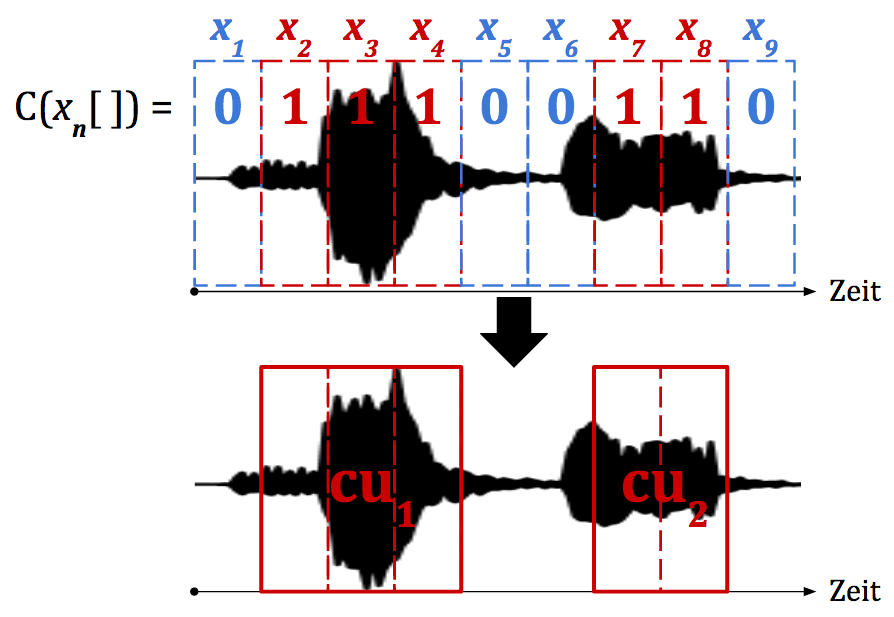
\includegraphics[width=0.6\textwidth]{bilder/cry-Unit02.png}
	\caption{Zusammenfassung klassifizierter Signalfenster zu Cry-Units}
	\label{img:cryUnit}
\end{figure}

Formel \ref{eq:cry-Unit} gibt die Definition des Datentypes \emph{Cry-Unit} [$CU$]. Eine Cry-Unit wird definiert durch den Anfangszeitpunkt $start$, einen Endzeitpunkt $end$ und der Liste seiner Signalfenster $windows = [x_0[\;], \ldots, x_n][\;]$.

\begin{equation}
CU = (windows = \big[x_0[\;] ,\ldots, x_n[\;] \big], start \in Zeit, end \in Zeit)
\label{eq:cry-Unit}
\end{equation}

Die Dauer eine Cry-Unit $cu \in CU$ wird nach Formel \ref{eq:cry-Lambda} berechnet und mit $\lambda$ bezeichnet. Die zeitliche Dauer der Pause zwischen zwei Cry-Units d($cu_i, cu_j$), wird nach Formel \ref{eq:cry-distance} berechnet. Diese Zusammenhänge werden in Abbildung \ref{img:cryUnit-details} visualisiert.\cite[S. 2]{vad_entropy}

\begin{equation}
\lambda (cu) = cu.end - cu.start
\label{eq:cry-Lambda}
\end{equation}

\begin{equation}
\text{d}(cu_i, cu_j) = cu_j.start - cu_i.end
\label{eq:cry-distance}
\end{equation}

\begin{figure}[h]
	\centering
	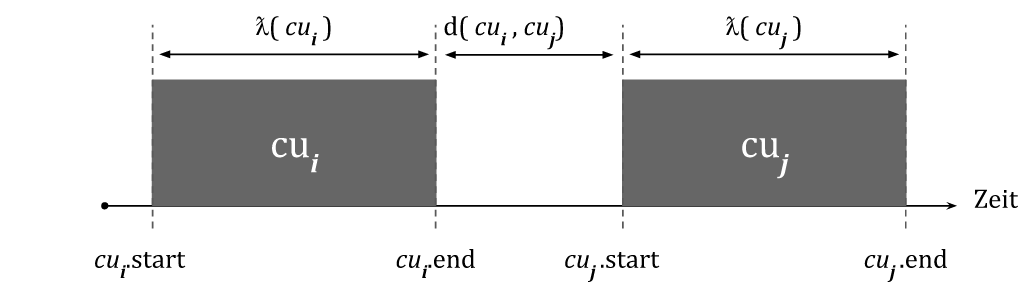
\includegraphics[width=0.8\textwidth]{bilder/newSmoothing05.png}
	\caption{Beziehung zwischen agrenzenden Cry-Units, nach \cite[S. 2]{vad_entropy}}
	\label{img:cryUnit-details}
\end{figure}

Algorithmus \ref{alg:cryUnit} zeigt in Pseudo-Code, wie auf Basis der Liste aller Signalfenster eines Signals $X_{all} = [x_0[\;] ,\ldots, x_m[\;]]$ die Liste der Cry-Units $CU_{all}$ generiert wird. Die Funktion $C(x[\;])$ ist die Klassifikations-Funktion der Signalfenster in Stille/Stimme nach Gleichung \ref{eq:vad-final}. Die Funktion getTimeOf$(x_i[\;])$ liefert die Anfangszeitpunkt des Signalfensters $x_i[\;]$.

\begin{algorithm}[h]
	\caption{Gruppierung von Signalfenstern zu Cry-Units}
	\label{alg:cryUnit}
	\begin{algorithmic}[1]
		\Function{turnWindowsIntoCryUnits}{$X_{all}$}
		\State $ CU_{all} \gets [\;]$
		\State $ cu\gets ([\;],0,0)$
		\For{\textbf{all} $x_i[\;] \in X_{all}$}
				\State $ c \gets C(x_i[\;])$
				\State \Comment Start of Cry-Unit
				\If {$c == 1 \wedge \text{isEmpty}(cu.windows)$}
						\State $cu\gets ([\;],0,0)$
						\State $cu.start \gets \text{getTimeOf}(x_i[\;])$
						\State $cu.windows \gets [cu.windows, x_i[\;]]$
				\EndIf
				\State \Comment Inside Cry-Unit
				\If {$c == 1 \wedge \text{ ! isEmpty}(cu.windows)$}
						\State $cu.windows \gets [cu.windows, x_i[\;]]$
				\EndIf
				\State \Comment End of Cry-Unit
				\If {$c == 0 \wedge \text{ ! isEmpty}(cu.windows)$}
						\State $cu.end \gets  getTimeOf(x_i[\;])$
						\State $CU \gets [CU, cu]$
						\State $cu.windows \gets [\;]$
				\EndIf
		\EndFor
		
		\State \Comment End last Cry-Unit by force if still open.
		\If {$\text{ ! isEmpty}(cu.windows) == 0$}
		\State $cu.end \gets  getTimeOf(X_{windows}[end])$
		\State $CU_{all} \gets [CU_{all}, cu]$
		\EndIf
		
		\Return $CU_{all}$
		
		\EndFunction
		
	\end{algorithmic}
\end{algorithm}

\subsection{Decision Smoothing}
\label{sec:smoothing}

Abbildung \ref{img:beforeSmoothing} zeigt ein Audiosignal mit einem Signal-Rausch-Abstand von \SI{3}{\decibel}, bei dem die Voice Activity Detection durchgeführt wurde. Die rote Linie zeigt die tatsächliche Klassifiikation und die grüne Linie die prognostizierte Klassifikation. Es ist zu sehen, dass einige False-Negatives und prongnostiziert wurden. Im folgenden werden drei charakteristische Arten falscher Klassifikationen näher erläutert:

\begin{description}
	\item [False Negatives nach (a): ] Eine korrekt erkannte, längere Cry-Unit wird zu früh beendet. Oft werden kurz nach dem Ende einer längeren Cry-Unit sehr kurze Cry-Units erkannt, die eigentlich noch zu der längeren, vorhergehenden Cry-Unit gehören.
	\item [False Positives nach (b): ] Kurze Cry-Units werden in eigentlichen Stille-Bereichen erkannt.
	\item [False Negatives nach (c): ] Eine Cry-Unit zerfällt in zwei Cry-Units, da kurze Signalfenster in der Mitte als Stille erkannt wurden.
\end{description}

\begin{figure}[h]
	\centering
	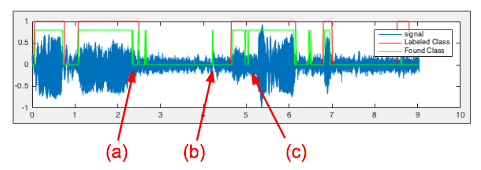
\includegraphics[width=0.7\textwidth]{bilder/smoothing02.png}
	\caption{Klassifizierung vor dem Decision Smoothing}
	\label{img:beforeSmoothing}
\end{figure}

Im Process des \textbf{Decision Smoothing} werden kontextuelle Informationen genutzt, um nachträglich False-Positives und False-Negatives zu entfernen. Es werden dazu die von Waheed et al \cite{vad_entropy} präsentierten Ideen verwendet. Es werden zwei Parameter eingeführt: $\lambda_{min}$, die Mindestlänge einer akzeptierten Cry-Unit, und d$_{min}$, die Mindestlänge eines akzeptierten Stille-Segmentes. Das Decision-Smoothing wird nach den folgenden Entscheidungsregeln durchgeführt:

\pagebreak
\noindent\rule{\linewidth}{0.3pt}
\begin{itemize}
	\item ist $\lambda (cu_{i}) \leq \lambda_{min}$ ?
	\begin{itemize}
		\item wenn $\lambda (cu_{i-1}) > \lambda_{min}$ und $d (cu_{i-1}, cu_{i}) \leq d_{min}$, dann vereinige $cu_{i}$ mit $cu_{i-1}$ . $\Longrightarrow$ behebt False-Negatives des Types (a)
		\item ansonsten entferne $cu_i \Longrightarrow$ behebt False-Negatives des Types (b)
	\end{itemize}
	\item wenn $\lambda (cu_{i}) > \lambda_{min}$ und $d (cu_{i-1}, cu_{i}) \leq d_{min}$, dann vereinige $cu_{i}$ mit $cu_{i-1}$ . $\Rightarrow$ behebt False-Negatives des Types (c)
\end{itemize}
\noindent\rule{\linewidth}{0.3pt}

Die Entscheidungsregeln greifen nur auf die letzten beiden erkannten Cry-Units zu, um eine kontinuierliche Analyse zu gewährleisten. Bei einer kontinuierlichen Analyse wird die Auswertung um die Zeitdauer einer Cry-Unit verzögert, da die Entscheidungsregeln erst nach Beendigung einer Cry-Unit abgefragt werden können. Bei einer offline-Analyse können die Entscheidungsregeln vereinfacht werden, da die False-Negatives nach Typ (a) und (c) mit der selben Regel abgefragt werden können. Algorithmus \ref{alg:decisionSmoothing} zeigt in Pseudo-Code, wie das Decision-Smoothing durchgeführt wird. Input der Funktion ist die Liste aller Cry-Units $CU_{all} = [cu_0 , \ldots , cu_n]$, die durch Algorithmus \ref{alg:cryUnit} entstanden ist, sowie die Grenzwerte $\lambda_{min}, d_{min}$. Der Output der Funktion ist die Liste aller Cry-Units nach dem Decision-Smoothing $CU_{smoothed}$.

\begin{algorithm}[h]
	\caption{Decision-Smoothing for VAD}
	\label{alg:decisionSmoothing}
	\begin{algorithmic}[1]
		\Function{decisionSmoothing}{$CU_{all}, \lambda_{min}, d_{min}$}
		\State $CU_{smoothed} \gets[CU_{all}[0]] $
		\State \Comment start for-loop at the \emph{second} cry-Unit!
		\For{ $i = 1 , \ldots , length(CU_{all}) - 1$}
			\State $cu_i \gets CU_{all}[i]$
			\State $cu_{i-1} \gets CU_{smoothed}[end]$
			\If{$\lambda(cu_i) > \lambda_{min}$}
			\State \Comment Accept Cry-Unit
			\If{d$(cu_{i-1},cu_{i}) > d_{min}$}
					\State $CU_{smoothed} \gets [CU_{smoothed}, cu_i] $
			\Else
					\State \Comment Erase False-Negative Type (c)
					\State $cu_i \gets \text{vereinige}(cu_i, cu_{i-1})$
					\State $CU_{smoothed} \gets [CU_{smoothed}[1:end-1], cu_i] $
			\EndIf
			\Else
			\State \Comment Erase False-Negative Type (a)
			\If{$d(cu_{i-1},cu_{i}) \leq d_{min}$ }
			\State $cu_i \gets \text{vereinige}(cu_i, cu_{i-1})$
			\State $CU_{smoothed} \gets [CU_{smoothed}[0:end-1], cu_i] $
			\Else
			\State \Comment Don't accept $cu_i$. Erases False-Positives (b)
			\EndIf
			\EndIf
		\EndFor
		
		\Return $CU_{smoothed}$
		\EndFunction
		
	\end{algorithmic}
\end{algorithm}

Abbildung \ref{img:after-smoothing} zeigt das Beispielsignal vor und nach dem Decision-Smoothing. In verschiedenen Veröffentlichungen wurden unterschiedliche Mindestlängen von Cry-Units festgestellt. Varallyay \cite[S. 8]{cry_thesis} hat beispielsweise eine Mindestlänge von \SI{250}{\milli\second} gemessen. Der geringste Wert, der nach dem Wissen des Autors in einer Veröffentlichung genannt wurde, stammt von Zeskind et al \cite[S. 325]{rythmic} und beträgt  \SI{60}{\milli\second}, welcher für $\lambda_{min}$ übernommen wurde. Es konnten hingegen keine Werte über die geringste festgestellte Pause zwischen zwei Cry-Units gefunden werden. Der Wert wurde daher auf Basis des verwendeten Trainings-Datensatzes ebenfalls mit $d_{min} = \SI{60}{\milli\second}$ bestimmt. 

\begin{figure}[h]
	\centering
	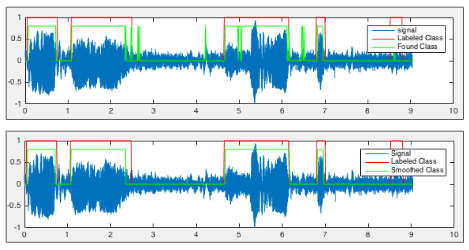
\includegraphics[width=0.6\textwidth]{bilder/smoothing04.png}
	\caption{Klassifikation vor und nach dem Decision Smoothing}
	\label{img:after-smoothing}
\end{figure}

\subsection{Diskussion der Voice-Activity-Detection}

In diesem Kapitel wurden verschiedene Methoden der Voice Activity Detection vorgestellt, verglichen und evaluiert, wobei eine Voice Activity Detection auf Basis des Cepstrums die besten Ergebnisse erzielte. Unabhängig von den konkret verglichenen Features werden in dieser grundlegenden Herangehensweise zur Voice Activity Detection kontextuelle Informationen in Bezug auf den zeitlichen Verlauf der Stimme jedoch nur in einem geringen Maße beim Decision-Smoothing verwertet. Schlussendlich markiert der VAD-Algorithmus eine Reihe von kurzen Signalfenstern genau dann als zusammenhängende Cry-Unit, wenn jedes Signalfenster für sich betrachtet als Lautäußerung eines Babies klassifiziert wurde. Ob jedoch die Reihenfolge der in den Signalfenstern enthaltenen Lautäußerungen Sinn macht, wird nicht betrachtet. Schneidet man beispielsweise wenige Sekunden aus der Mitte einer längeren Cry-Unit aus und konkateniert dieses Sample viele Male, um eine synthetische, längere Cry-Unit zu erzeugen, klingt das Ergebnis für den Menschen stark unnatürlich, wird von dem hier vorgestellten VAD-Algorithmus jedoch trotzdem als valide Cry-Unit markiert. Das Cepstrum als Feature mit der höchsten Accuracy ist somit so zu bewerten, dass es vor allem im geringen Maße kontextuell Informationen benötigt, um eine Entscheidung über das vorahndensein von Stimme zu fällen. Zukünftige Forschungen könnnen an diesem Punkt ansetzen, um die Accuracy der VAD zu erhöhen.